%!TeX root = main.tex
\section{Report of 2024 05 13}

The compute shader which was taking 24.15 ms for 1M particles now performs the same in 5.09ms. The improvement results from fixing a recursive bug.
(Compare \figo{GPUTrace001},\figo{GPUTrace})


\input{../images/GPUTrace001.tex}
\input{../images/GPUTrace.tex}

\Figo{GPUTrace001} also suggests possible further performance enhancements. The compute is cyclical and not fully utilizing the GPU. There is a large break 
in the graphics pipeline. Both compute and graphics pipelines are not yet fully threaded.  

Table \ref{tab:V-Cube Performance Data} shows improvement across the board (with reference to table \ref{tab:V-Cube Performance Data001}). One million particles are now 
processed at 78 fps. \Figo{Perf_VCUBE02} is greatly improved and appears linear. The red line is a linear fit. The green line is $0.5E-8x$ where x is the number of particles. 
I am trying to display the linear line. The fit line is above this so the relationship is \q{super linear?}.

There are two types of density. The first is the particle density which is the ratio of the number of particles in a cell to the maximum 
number of particles that can fit in a cell $\frac{cell\quad population}{max\quad cell\quad population}$. The maximum number of particles 
that can fit in a cell depends on the radius of the particles. In the current case the \textit{max cell population} is 30. The collision density is the number of 
collisions divided by the number of particles in a cell $\frac{number\quad collisions\quad in\quad cell}{cell\quad population}$.   

I have included a section on how the bench-marking/verification is done. One of the problems I had in reviewing particle collision detection is that 
the number of collisions in the data was not verified against the number of collisions the method detected. I do this verification so the numbers here
are starting to have credibility. \q{although I am not sure I understand them completely}.


\input{../tables/V-Cube Performance Data.tex}

\input{../tables/V-Cube Performance Data001.tex}


\begin{figure}[h]
\centering
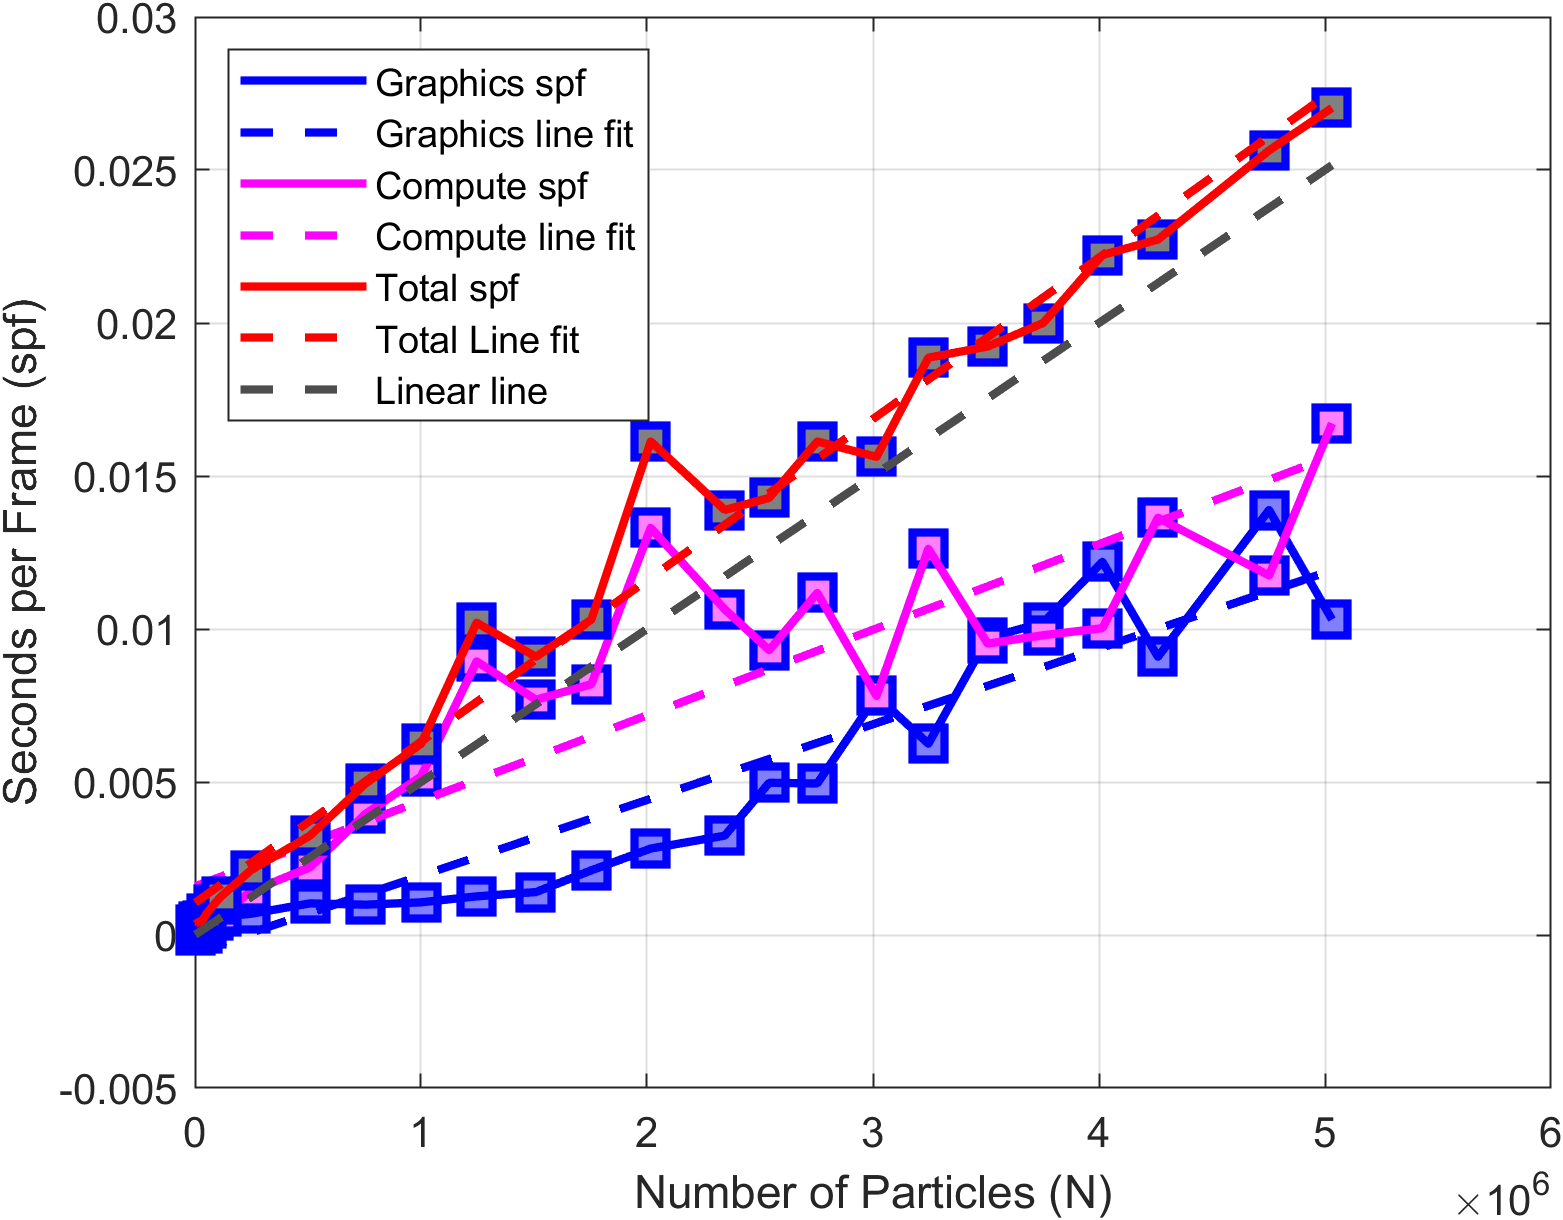
\includegraphics[width=2.97in]{../plots/Perf_VCUBE021.png}
\captionof{figure}[FPS Performance Data]{Seconds per frame for 0.5 collision density with 30 particles per cell verses number of particles.}
\label{fig:Perf_VCUBE02}
\end{figure}

\begin{figure}[h]
\centering
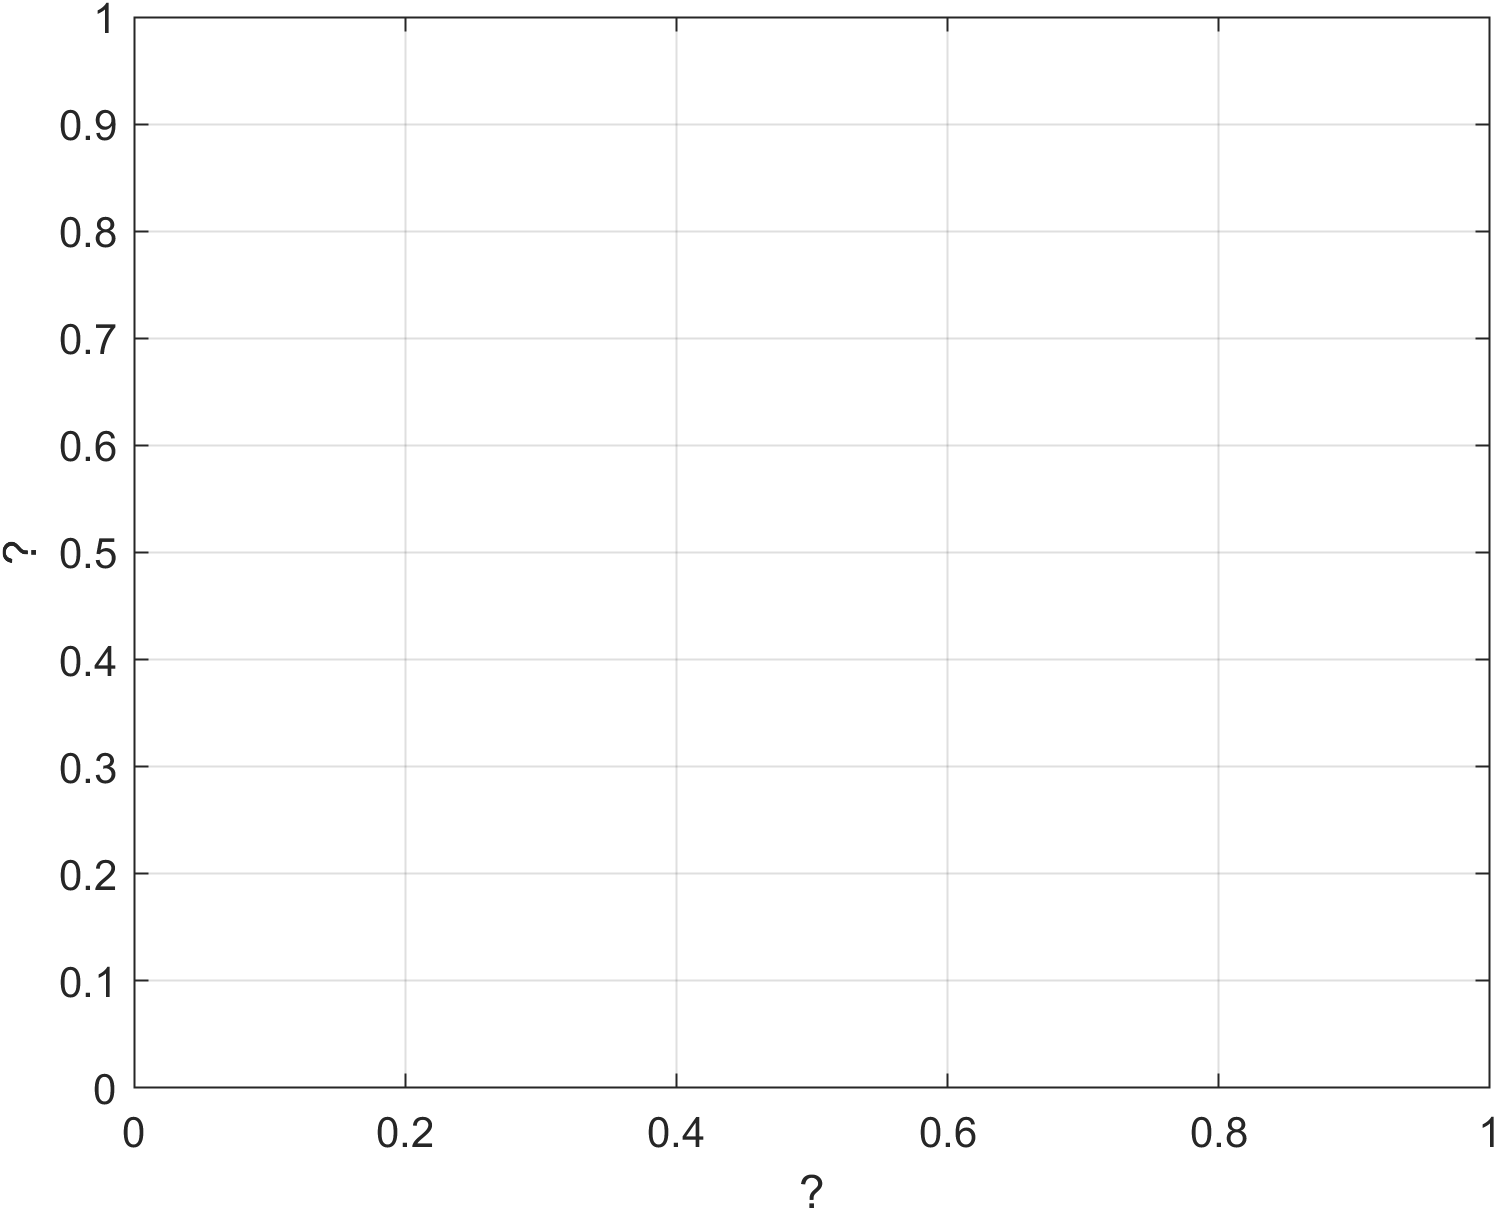
\includegraphics[width=2.97in]{../plots/Perf_VCUBE041.png}
\captionof{figure}[Frame time divided by number of particles.]{CCP number of collisions divided by number of particles for 0.5 collision density with 30 particles per cell verses number of particles.}
\label{fig:Perf_VCUBE04}
\end{figure}

\newpage
\clearpage
%\newpage
%\input{../tables/V-Cube Performance Data.tex}
%\newpage
%\input{../tables/V-Cube Performance Data001.tex}
%\newpage
%\begin{figure}[h]
\centering
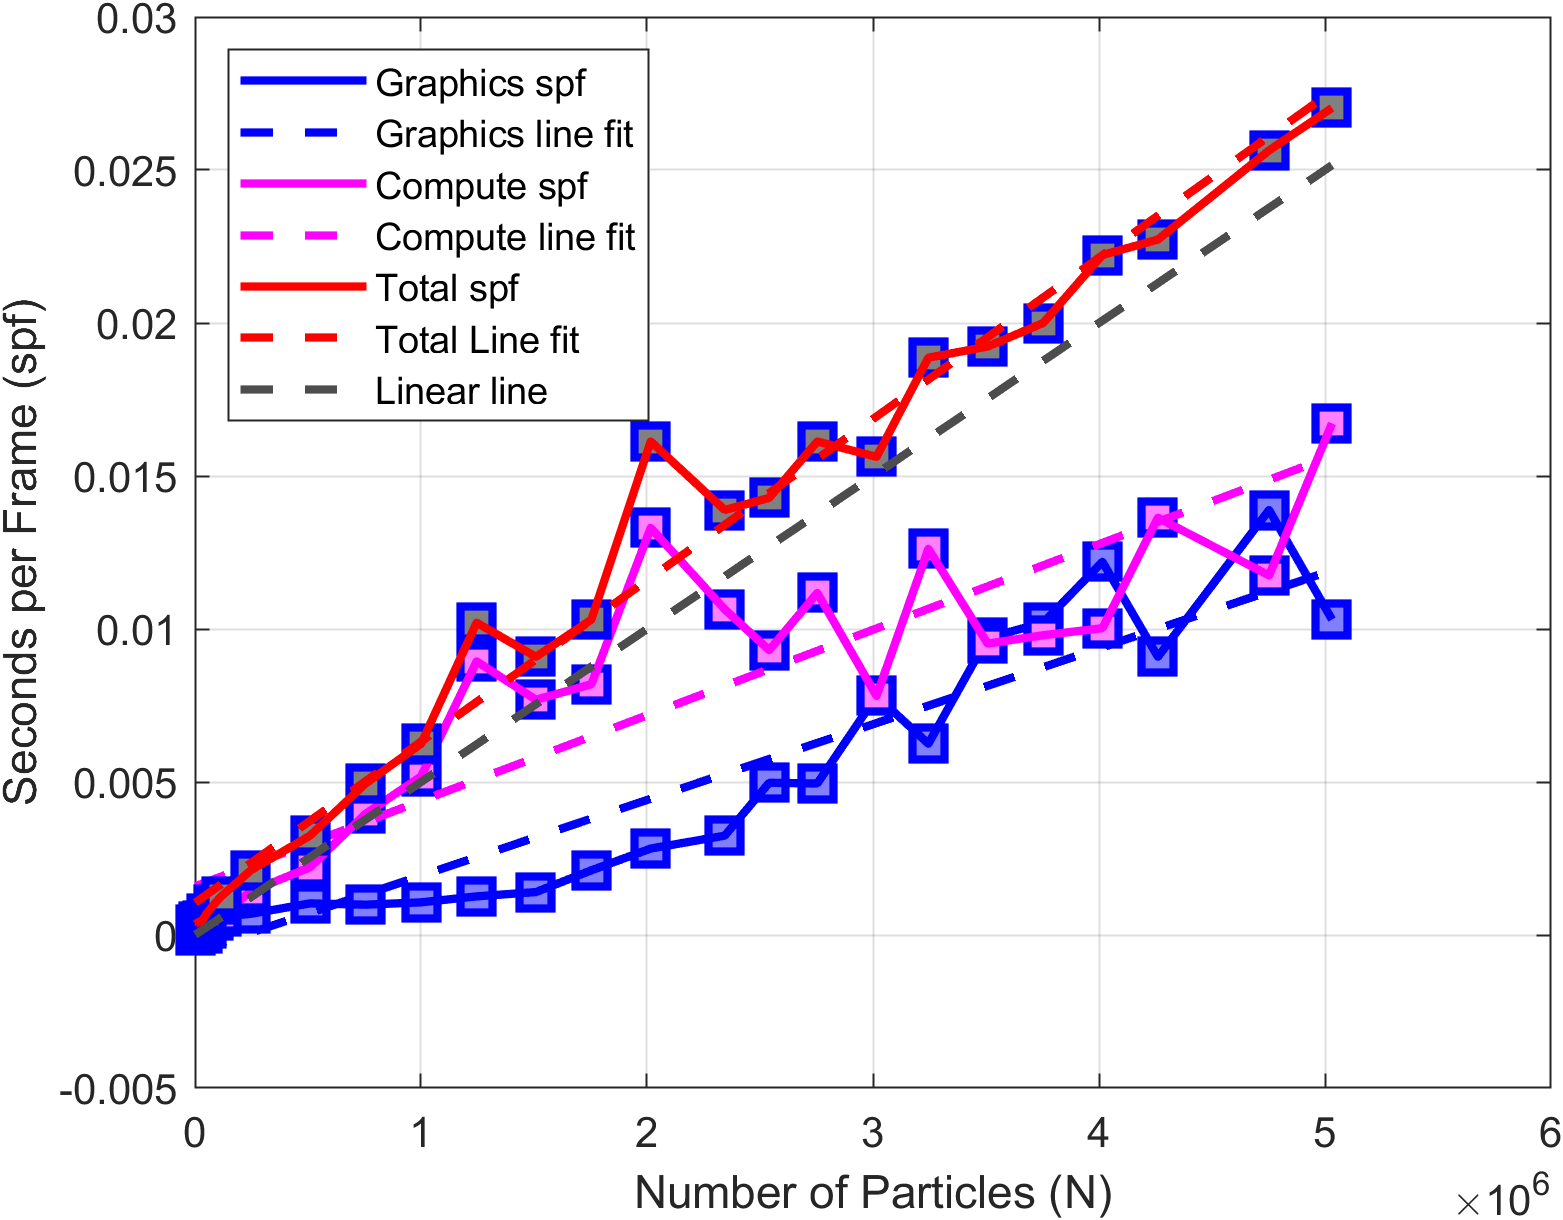
\includegraphics[width=2.97in]{../plots/Perf_VCUBE021.png}
\captionof{figure}[FPS Performance Data]{Seconds per frame for 0.5 collision density with 30 particles per cell verses number of particles.}
\label{fig:Perf_VCUBE02}
\end{figure}

%\begin{figure}[h]
\centering
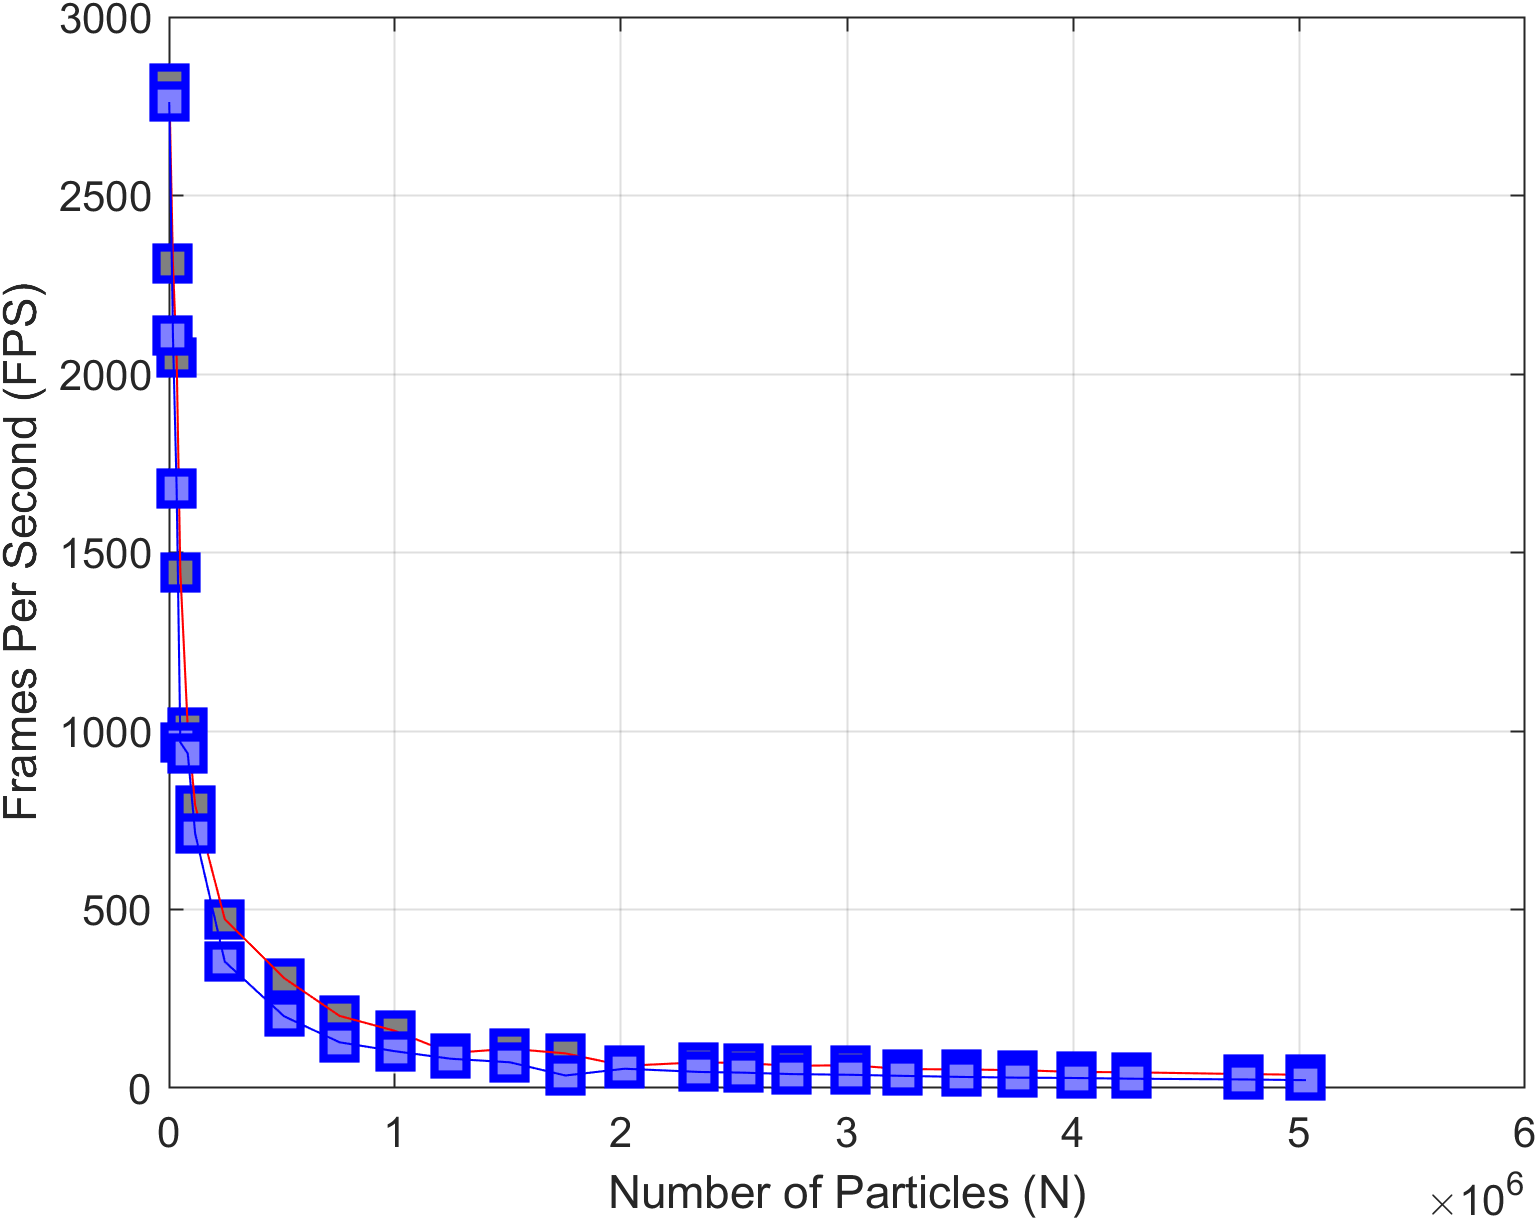
\includegraphics[width=2.97in]{../plots/Perf_VCUBE011.png}
\captionof{figure}[SPf Performance Data]{Frames per second for 0.5 collision density with 30 particles per cell verses number of particles.}
\label{fig:Perf_VCUBE01}
\end{figure}


%\begin{figure}[h]
\centering
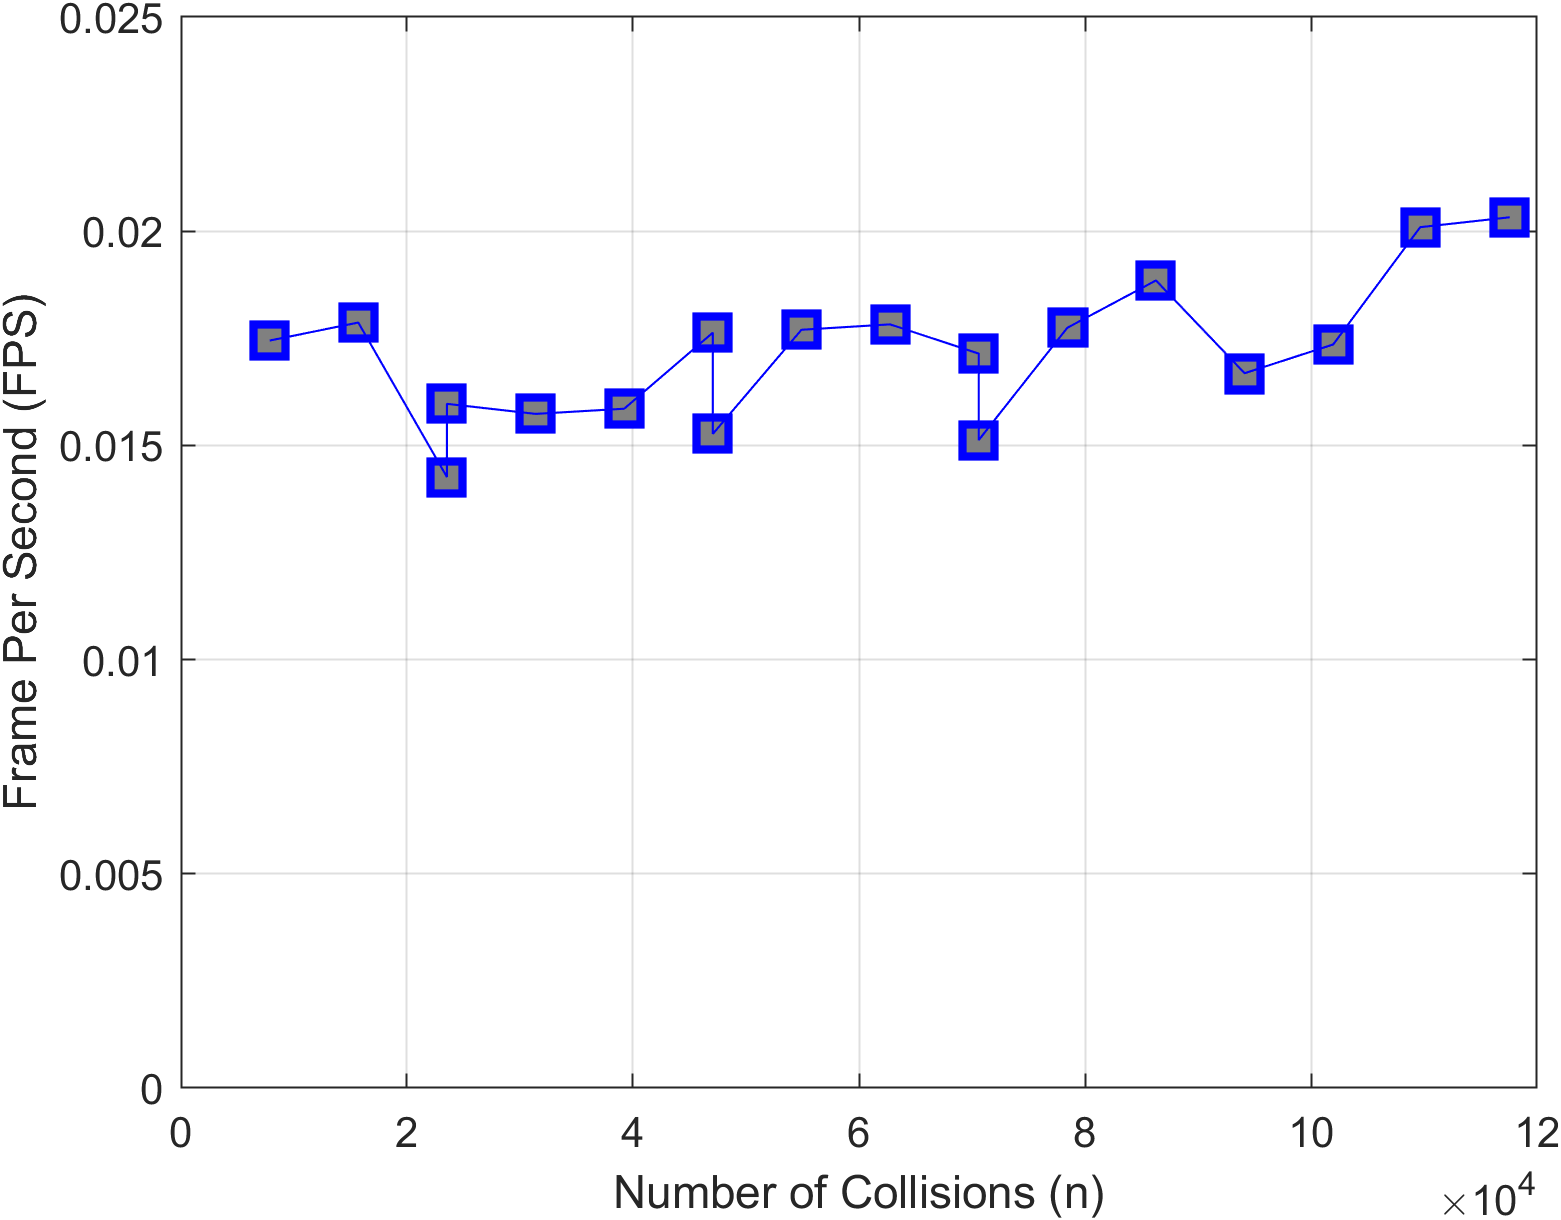
\includegraphics[width=2.97in]{../plots/Perf_RCPCD_Density0011.png}
\captionof{figure}[Frame rate verses density of collisions at 117,650 particles particles and density 0.1-1.0..]{Frame rate verses density of collisions at 117,650 particles and density from 10-100\%}
\label{fig:Perf_RCPCD_Density001}
\end{figure}


%\begin{figure}[h]
\centering
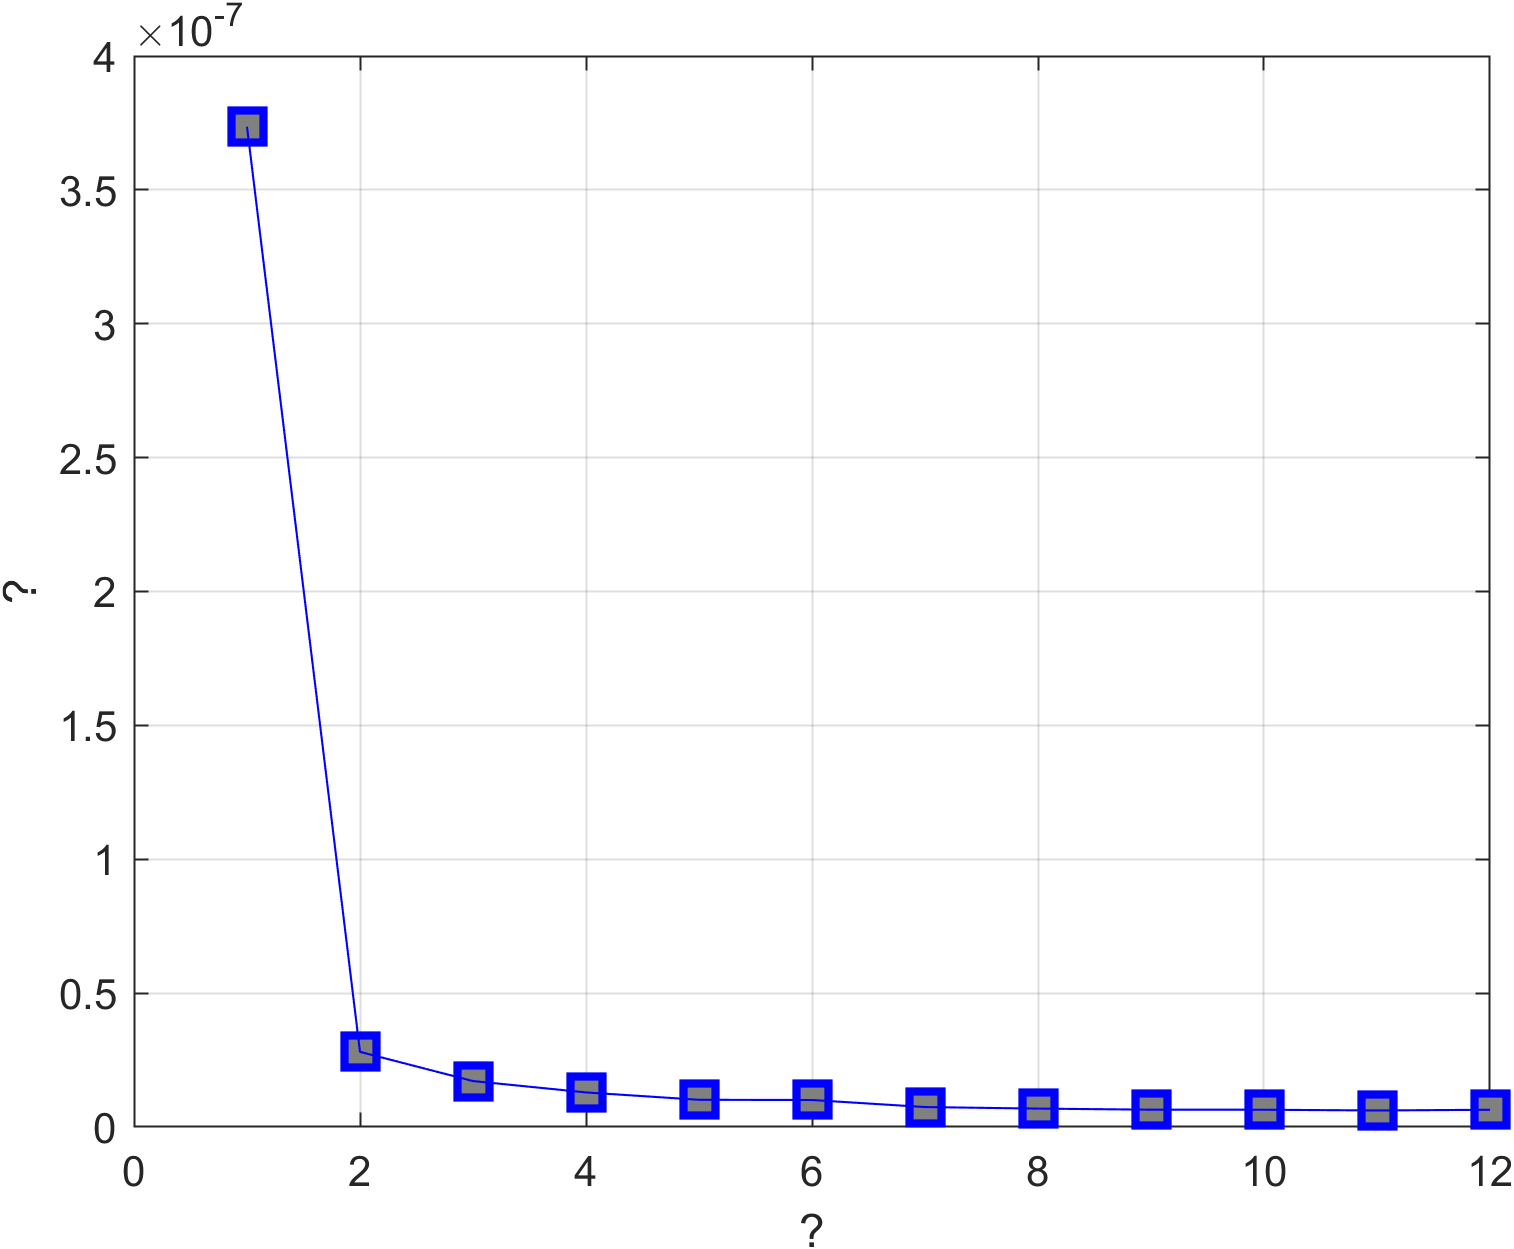
\includegraphics[width=2.97in]{../plots/Perf_VCUBE031.png}
\captionof{figure}[Linearity.]{Linearity - Frame time divided by number of particles for 0.5 collision density with 30 particles per cell verses number of particles.}
\label{fig:Perf_VCUBE03}
\end{figure}


%\begin{figure}[h]
\centering
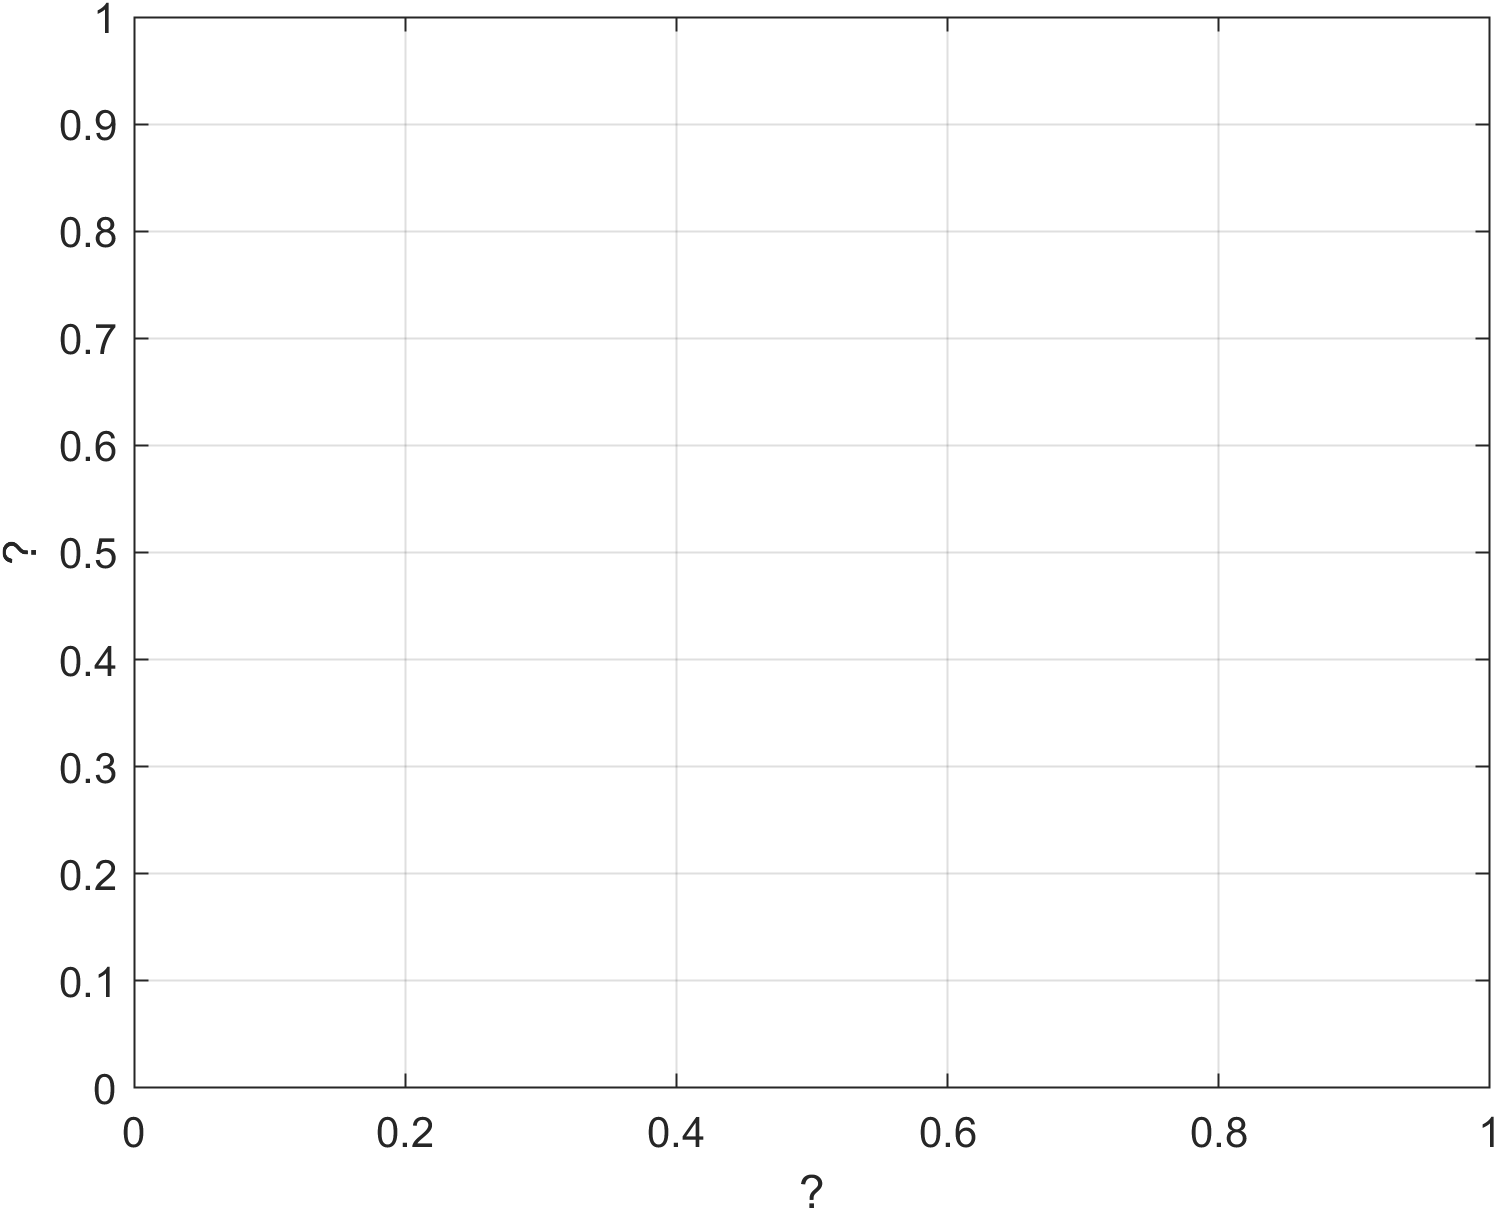
\includegraphics[width=2.97in]{../plots/Perf_VCUBE041.png}
\captionof{figure}[Frame time divided by number of particles.]{CCP number of collisions divided by number of particles for 0.5 collision density with 30 particles per cell verses number of particles.}
\label{fig:Perf_VCUBE04}
\end{figure}

%Fig. \ref{fig:Perf_RCPCD_Density001}

